\documentclass[1p]{elsarticle_modified}
%\bibliographystyle{elsarticle-num}

%\usepackage[colorlinks]{hyperref}
%\usepackage{abbrmath_seonhwa} %\Abb, \Ascr, \Acal ,\Abf, \Afrak
\usepackage{amsfonts}
\usepackage{amssymb}
\usepackage{amsmath}
\usepackage{amsthm}
\usepackage{scalefnt}
\usepackage{amsbsy}
\usepackage{kotex}
\usepackage{caption}
\usepackage{subfig}
\usepackage{color}
\usepackage{graphicx}
\usepackage{xcolor} %% white, black, red, green, blue, cyan, magenta, yellow
\usepackage{float}
\usepackage{setspace}
\usepackage{hyperref}

\usepackage{tikz}
\usetikzlibrary{arrows}

\usepackage{multirow}
\usepackage{array} % fixed length table
\usepackage{hhline}

%%%%%%%%%%%%%%%%%%%%%
\makeatletter
\renewcommand*\env@matrix[1][\arraystretch]{%
	\edef\arraystretch{#1}%
	\hskip -\arraycolsep
	\let\@ifnextchar\new@ifnextchar
	\array{*\c@MaxMatrixCols c}}
\makeatother %https://tex.stackexchange.com/questions/14071/how-can-i-increase-the-line-spacing-in-a-matrix
%%%%%%%%%%%%%%%

\usepackage[normalem]{ulem}

\newcommand{\msout}[1]{\ifmmode\text{\sout{\ensuremath{#1}}}\else\sout{#1}\fi}
%SOURCE: \msout is \stkout macro in https://tex.stackexchange.com/questions/20609/strikeout-in-math-mode

\newcommand{\cancel}[1]{
	\ifmmode
	{\color{red}\msout{#1}}
	\else
	{\color{red}\sout{#1}}
	\fi
}

\newcommand{\add}[1]{
	{\color{blue}\uwave{#1}}
}

\newcommand{\replace}[2]{
	\ifmmode
	{\color{red}\msout{#1}}{\color{blue}\uwave{#2}}
	\else
	{\color{red}\sout{#1}}{\color{blue}\uwave{#2}}
	\fi
}

\newcommand{\Sol}{\mathcal{S}} %segment
\newcommand{\D}{D} %diagram
\newcommand{\A}{\mathcal{A}} %arc


%%%%%%%%%%%%%%%%%%%%%%%%%%%%%5 test

\def\sl{\operatorname{\textup{SL}}(2,\Cbb)}
\def\psl{\operatorname{\textup{PSL}}(2,\Cbb)}
\def\quan{\mkern 1mu \triangleright \mkern 1mu}

\theoremstyle{definition}
\newtheorem{thm}{Theorem}[section]
\newtheorem{prop}[thm]{Proposition}
\newtheorem{lem}[thm]{Lemma}
\newtheorem{ques}[thm]{Question}
\newtheorem{cor}[thm]{Corollary}
\newtheorem{defn}[thm]{Definition}
\newtheorem{exam}[thm]{Example}
\newtheorem{rmk}[thm]{Remark}
\newtheorem{alg}[thm]{Algorithm}

\newcommand{\I}{\sqrt{-1}}
\begin{document}

%\begin{frontmatter}
%
%\title{Boundary parabolic representations of knots up to 8 crossings}
%
%%% Group authors per affiliation:
%\author{Yunhi Cho} 
%\address{Department of Mathematics, University of Seoul, Seoul, Korea}
%\ead{yhcho@uos.ac.kr}
%
%
%\author{Seonhwa Kim} %\fnref{s_kim}}
%\address{Center for Geometry and Physics, Institute for Basic Science, Pohang, 37673, Korea}
%\ead{ryeona17@ibs.re.kr}
%
%\author{Hyuk Kim}
%\address{Department of Mathematical Sciences, Seoul National University, Seoul 08826, Korea}
%\ead{hyukkim@snu.ac.kr}
%
%\author{Seokbeom Yoon}
%\address{Department of Mathematical Sciences, Seoul National University, Seoul, 08826,  Korea}
%\ead{sbyoon15@snu.ac.kr}
%
%\begin{abstract}
%We find all boundary parabolic representation of knots up to 8 crossings.
%
%\end{abstract}
%\begin{keyword}
%    \MSC[2010] 57M25 
%\end{keyword}
%
%\end{frontmatter}

%\linenumbers
%\tableofcontents
%
\newcommand\colored[1]{\textcolor{white}{\rule[-0.35ex]{0.8em}{1.4ex}}\kern-0.8em\color{red} #1}%
%\newcommand\colored[1]{\textcolor{white}{ #1}\kern-2.17ex	\textcolor{white}{ #1}\kern-1.81ex	\textcolor{white}{ #1}\kern-2.15ex\color{red}#1	}

{\Large $\underline{12a_{1081}~(K12a_{1081})}$}

\setlength{\tabcolsep}{10pt}
\renewcommand{\arraystretch}{1.6}
\vspace{1cm}\begin{tabular}{m{100pt}>{\centering\arraybackslash}m{274pt}}
\multirow{5}{120pt}{
	\centering
	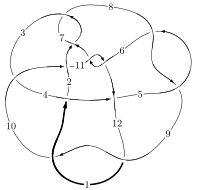
\includegraphics[width=112pt]{../../../GIT/diagram.site/Diagrams/png/1882_12a_1081.png}\\
\ \ \ A knot diagram\footnotemark}&
\allowdisplaybreaks
\textbf{Linearized knot diagam} \\
\cline{2-2}
 &
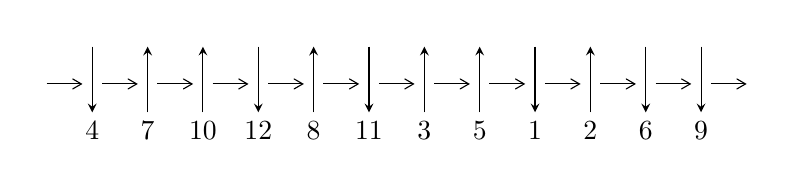
\begin{tikzpicture}[x=20pt, y=17pt]
	% nodes
	\node (C0) at (0, 0) {};
	\node (C1) at (1, 0) {};
	\node (C1U) at (1, +1) {};
	\node (C1D) at (1, -1) {4};

	\node (C2) at (2, 0) {};
	\node (C2U) at (2, +1) {};
	\node (C2D) at (2, -1) {7};

	\node (C3) at (3, 0) {};
	\node (C3U) at (3, +1) {};
	\node (C3D) at (3, -1) {10};

	\node (C4) at (4, 0) {};
	\node (C4U) at (4, +1) {};
	\node (C4D) at (4, -1) {12};

	\node (C5) at (5, 0) {};
	\node (C5U) at (5, +1) {};
	\node (C5D) at (5, -1) {8};

	\node (C6) at (6, 0) {};
	\node (C6U) at (6, +1) {};
	\node (C6D) at (6, -1) {11};

	\node (C7) at (7, 0) {};
	\node (C7U) at (7, +1) {};
	\node (C7D) at (7, -1) {3};

	\node (C8) at (8, 0) {};
	\node (C8U) at (8, +1) {};
	\node (C8D) at (8, -1) {5};

	\node (C9) at (9, 0) {};
	\node (C9U) at (9, +1) {};
	\node (C9D) at (9, -1) {1};

	\node (C10) at (10, 0) {};
	\node (C10U) at (10, +1) {};
	\node (C10D) at (10, -1) {2};

	\node (C11) at (11, 0) {};
	\node (C11U) at (11, +1) {};
	\node (C11D) at (11, -1) {6};

	\node (C12) at (12, 0) {};
	\node (C12U) at (12, +1) {};
	\node (C12D) at (12, -1) {9};
	\node (C13) at (13, 0) {};

	% arrows
	\draw[->,>={angle 60}]
	(C0) edge (C1) (C1) edge (C2) (C2) edge (C3) (C3) edge (C4) (C4) edge (C5) (C5) edge (C6) (C6) edge (C7) (C7) edge (C8) (C8) edge (C9) (C9) edge (C10) (C10) edge (C11) (C11) edge (C12) (C12) edge (C13) ;	\draw[->,>=stealth]
	(C1U) edge (C1D) (C2D) edge (C2U) (C3D) edge (C3U) (C4U) edge (C4D) (C5D) edge (C5U) (C6U) edge (C6D) (C7D) edge (C7U) (C8D) edge (C8U) (C9U) edge (C9D) (C10D) edge (C10U) (C11U) edge (C11D) (C12U) edge (C12D) ;
	\end{tikzpicture} \\
\hhline{~~} \\& 
\textbf{Solving Sequence} \\ \cline{2-2} 
 &
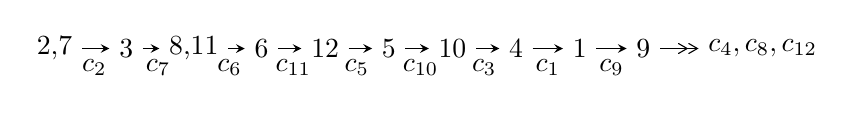
\begin{tikzpicture}[x=23pt, y=7pt]
	% node
	\node (A0) at (-1/8, 0) {2,7};
	\node (A1) at (1, 0) {3};
	\node (A2) at (33/16, 0) {8,11};
	\node (A3) at (25/8, 0) {6};
	\node (A4) at (33/8, 0) {12};
	\node (A5) at (41/8, 0) {5};
	\node (A6) at (49/8, 0) {10};
	\node (A7) at (57/8, 0) {4};
	\node (A8) at (65/8, 0) {1};
	\node (A9) at (73/8, 0) {9};
	\node (C1) at (1/2, -1) {$c_{2}$};
	\node (C2) at (3/2, -1) {$c_{7}$};
	\node (C3) at (21/8, -1) {$c_{6}$};
	\node (C4) at (29/8, -1) {$c_{11}$};
	\node (C5) at (37/8, -1) {$c_{5}$};
	\node (C6) at (45/8, -1) {$c_{10}$};
	\node (C7) at (53/8, -1) {$c_{3}$};
	\node (C8) at (61/8, -1) {$c_{1}$};
	\node (C9) at (69/8, -1) {$c_{9}$};
	\node (A10) at (11, 0) {$c_{4},c_{8},c_{12}$};

	% edge
	\draw[->,>=stealth]	
	(A0) edge (A1) (A1) edge (A2) (A2) edge (A3) (A3) edge (A4) (A4) edge (A5) (A5) edge (A6) (A6) edge (A7) (A7) edge (A8) (A8) edge (A9) ;
	\draw[->>,>={angle 60}]	
	(A9) edge (A10);
\end{tikzpicture} \\ 

\end{tabular} \\

\footnotetext{
The image of knot diagram is generated by the software ``\textbf{Draw programme}" developed by Andrew Bartholomew(\url{http://www.layer8.co.uk/maths/draw/index.htm\#Running-draw}), where we modified some parts for our purpose(\url{https://github.com/CATsTAILs/LinksPainter}).
}\phantom \\ \newline 
\centering \textbf{Ideals for irreducible components\footnotemark of $X_{\text{par}}$} 
 
\begin{align*}
I^u_{1}&=\langle 
-6.71552\times10^{713} u^{137}+1.22208\times10^{714} u^{136}+\cdots+1.77498\times10^{715} b-8.44541\times10^{717},\\
\phantom{I^u_{1}}&\phantom{= \langle  }2.38801\times10^{718} u^{137}+1.12887\times10^{718} u^{136}+\cdots+2.83805\times10^{719} a-1.43193\times10^{723},\\
\phantom{I^u_{1}}&\phantom{= \langle  }u^{138}- u^{137}+\cdots-38969 u+39973\rangle \\
I^u_{2}&=\langle 
-1.96664\times10^{19} u^{29}+4.76700\times10^{18} u^{28}+\cdots+1.93126\times10^{18} b-2.16039\times10^{19},\\
\phantom{I^u_{2}}&\phantom{= \langle  }-1.12071\times10^{18} u^{29}-4.65424\times10^{18} u^{28}+\cdots+7.72503\times10^{17} a+1.15956\times10^{19},\;u^{30}-5 u^{28}+\cdots+3 u+1\rangle \\
\\
\end{align*}
\raggedright * 2 irreducible components of $\dim_{\mathbb{C}}=0$, with total 168 representations.\\
\footnotetext{All coefficients of polynomials are rational numbers. But the coefficients are sometimes approximated in decimal forms when there is not enough margin.}
\newpage
\renewcommand{\arraystretch}{1}
\centering \section*{I. $I^u_{1}= \langle -6.72\times10^{713} u^{137}+1.22\times10^{714} u^{136}+\cdots+1.77\times10^{715} b-8.45\times10^{717},\;2.39\times10^{718} u^{137}+1.13\times10^{718} u^{136}+\cdots+2.84\times10^{719} a-1.43\times10^{723},\;u^{138}- u^{137}+\cdots-38969 u+39973 \rangle$}
\flushleft \textbf{(i) Arc colorings}\\
\begin{tabular}{m{7pt} m{180pt} m{7pt} m{180pt} }
\flushright $a_{2}=$&$\begin{pmatrix}1\\0\end{pmatrix}$ \\
\flushright $a_{7}=$&$\begin{pmatrix}0\\u\end{pmatrix}$ \\
\flushright $a_{3}=$&$\begin{pmatrix}1\\- u^2\end{pmatrix}$ \\
\flushright $a_{8}=$&$\begin{pmatrix}u\\- u^3+u\end{pmatrix}$ \\
\flushright $a_{11}=$&$\begin{pmatrix}-0.0841427 u^{137}-0.0397762 u^{136}+\cdots-1556.39 u+5045.49\\0.0378343 u^{137}-0.0688504 u^{136}+\cdots-2935.59 u+475.803\end{pmatrix}$ \\
\flushright $a_{6}=$&$\begin{pmatrix}-0.00948334 u^{137}+0.0136277 u^{136}+\cdots+823.451 u+2078.34\\-0.125302 u^{137}+0.0935960 u^{136}+\cdots+3676.61 u+1770.16\end{pmatrix}$ \\
\flushright $a_{12}=$&$\begin{pmatrix}0.704121 u^{137}-0.0203105 u^{136}+\cdots-1419.49 u-28148.0\\-0.00997754 u^{137}-0.00245078 u^{136}+\cdots-58.2883 u-451.123\end{pmatrix}$ \\
\flushright $a_{5}=$&$\begin{pmatrix}0.0611026 u^{137}-0.0773930 u^{136}+\cdots-2719.78 u+2720.21\\-0.122978 u^{137}+0.0948035 u^{136}+\cdots+3751.24 u+1595.19\end{pmatrix}$ \\
\flushright $a_{10}=$&$\begin{pmatrix}-0.121977 u^{137}+0.0290742 u^{136}+\cdots+1379.20 u+4569.68\\0.0378343 u^{137}-0.0688504 u^{136}+\cdots-2935.59 u+475.803\end{pmatrix}$ \\
\flushright $a_{4}=$&$\begin{pmatrix}-0.0294149 u^{137}-0.133869 u^{136}+\cdots-5251.86 u+4848.39\\0.0378481 u^{137}+0.0929219 u^{136}+\cdots+3476.87 u-5619.06\end{pmatrix}$ \\
\flushright $a_{1}=$&$\begin{pmatrix}0.232272 u^{137}-0.0507081 u^{136}+\cdots-1502.79 u-8678.55\\0.0517901 u^{137}-0.0821151 u^{136}+\cdots-3701.95 u+2195.58\end{pmatrix}$ \\
\flushright $a_{9}=$&$\begin{pmatrix}0.477195 u^{137}+0.0337432 u^{136}+\cdots+367.793 u-21597.4\\-0.0262764 u^{137}+0.0591113 u^{136}+\cdots+2863.72 u-1195.39\end{pmatrix}$\\&\end{tabular}
\flushleft \textbf{(ii) Obstruction class $= -1$}\\~\\
\flushleft \textbf{(iii) Cusp Shapes $= -0.288478 u^{137}+0.0182579 u^{136}+\cdots+166.945 u+9522.21$}\\~\\
\newpage\renewcommand{\arraystretch}{1}
\flushleft \textbf{(iv) u-Polynomials at the component}\newline \\
\begin{tabular}{m{50pt}|m{274pt}}
Crossings & \hspace{64pt}u-Polynomials at each crossing \\
\hline $$\begin{aligned}c_{1}\end{aligned}$$&$\begin{aligned}
&5(5 u^{138}-70 u^{137}+\cdots-54 u+1)
\end{aligned}$\\
\hline $$\begin{aligned}c_{2},c_{7}\end{aligned}$$&$\begin{aligned}
&u^{138}+u^{137}+\cdots+38969 u+39973
\end{aligned}$\\
\hline $$\begin{aligned}c_{3}\end{aligned}$$&$\begin{aligned}
&u^{138}+u^{137}+\cdots+11328 u+688
\end{aligned}$\\
\hline $$\begin{aligned}c_{4}\end{aligned}$$&$\begin{aligned}
&u^{138}+3 u^{137}+\cdots+1824290 u+445340
\end{aligned}$\\
\hline $$\begin{aligned}c_{5},c_{8}\end{aligned}$$&$\begin{aligned}
&5(5 u^{138}+20 u^{137}+\cdots+566 u+1601)
\end{aligned}$\\
\hline $$\begin{aligned}c_{6},c_{11}\end{aligned}$$&$\begin{aligned}
&u^{138}- u^{137}+\cdots+3352910 u+356879
\end{aligned}$\\
\hline $$\begin{aligned}c_{9},c_{12}\end{aligned}$$&$\begin{aligned}
&u^{138}+3 u^{137}+\cdots+35 u+293
\end{aligned}$\\
\hline $$\begin{aligned}c_{10}\end{aligned}$$&$\begin{aligned}
&5(5 u^{138}-15 u^{137}+\cdots-8.52426\times10^{8} u+2.04508\times10^{8})
\end{aligned}$\\
\hline
\end{tabular}\\~\\
\newpage\renewcommand{\arraystretch}{1}
\flushleft \textbf{(v) Riley Polynomials at the component}\newline \\
\begin{tabular}{m{50pt}|m{274pt}}
Crossings & \hspace{64pt}Riley Polynomials at each crossing \\
\hline $$\begin{aligned}c_{1}\end{aligned}$$&$\begin{aligned}
&25(25 y^{138}+220 y^{137}+\cdots-208 y+1)
\end{aligned}$\\
\hline $$\begin{aligned}c_{2},c_{7}\end{aligned}$$&$\begin{aligned}
&y^{138}-81 y^{137}+\cdots-16606311865 y+1597840729
\end{aligned}$\\
\hline $$\begin{aligned}c_{3}\end{aligned}$$&$\begin{aligned}
&y^{138}+21 y^{137}+\cdots+88302848 y+473344
\end{aligned}$\\
\hline $$\begin{aligned}c_{4}\end{aligned}$$&$\begin{aligned}
&y^{138}-45 y^{137}+\cdots-10148860553420 y+198327715600
\end{aligned}$\\
\hline $$\begin{aligned}c_{5},c_{8}\end{aligned}$$&$\begin{aligned}
&25(25 y^{138}+2770 y^{137}+\cdots+9.04133\times10^{8} y+2563201)
\end{aligned}$\\
\hline $$\begin{aligned}c_{6},c_{11}\end{aligned}$$&$\begin{aligned}
&y^{138}+103 y^{137}+\cdots+1941665805688 y+127362620641
\end{aligned}$\\
\hline $$\begin{aligned}c_{9},c_{12}\end{aligned}$$&$\begin{aligned}
&y^{138}-109 y^{137}+\cdots+451753 y+85849
\end{aligned}$\\
\hline $$\begin{aligned}c_{10}\end{aligned}$$&$\begin{aligned}
&25(25 y^{138}-1795 y^{137}+\cdots-1.65727\times10^{18} y+4.18236\times10^{16})
\end{aligned}$\\
\hline
\end{tabular}\\~\\
\newpage\flushleft \textbf{(vi) Complex Volumes and Cusp Shapes}
$$\begin{array}{c|c|c}  
\text{Solutions to }I^u_{1}& \I (\text{vol} + \sqrt{-1}CS) & \text{Cusp shape}\\
 \hline 
\begin{aligned}
u &= -0.996983 + 0.016036 I \\
a &= -0.196561 + 1.103920 I \\
b &= \phantom{-}2.82578 + 0.40806 I\end{aligned}
 & -0.433411 - 0.065140 I & \phantom{-0.000000 } 0 \\ \hline\begin{aligned}
u &= -0.996983 - 0.016036 I \\
a &= -0.196561 - 1.103920 I \\
b &= \phantom{-}2.82578 - 0.40806 I\end{aligned}
 & -0.433411 + 0.065140 I & \phantom{-0.000000 } 0 \\ \hline\begin{aligned}
u &= -1.022530 + 0.051510 I \\
a &= \phantom{-}0.080646 - 1.132090 I \\
b &= -0.76871 - 1.55789 I\end{aligned}
 & \phantom{-}1.37724 - 0.93730 I & \phantom{-0.000000 } 0 \\ \hline\begin{aligned}
u &= -1.022530 - 0.051510 I \\
a &= \phantom{-}0.080646 + 1.132090 I \\
b &= -0.76871 + 1.55789 I\end{aligned}
 & \phantom{-}1.37724 + 0.93730 I & \phantom{-0.000000 } 0 \\ \hline\begin{aligned}
u &= \phantom{-}1.017890 + 0.143350 I \\
a &= \phantom{-}0.238571 - 1.029880 I \\
b &= -0.02209 - 1.84159 I\end{aligned}
 & \phantom{-}0.88004 + 4.56519 I & \phantom{-0.000000 } 0 \\ \hline\begin{aligned}
u &= \phantom{-}1.017890 - 0.143350 I \\
a &= \phantom{-}0.238571 + 1.029880 I \\
b &= -0.02209 + 1.84159 I\end{aligned}
 & \phantom{-}0.88004 - 4.56519 I & \phantom{-0.000000 } 0 \\ \hline\begin{aligned}
u &= \phantom{-}0.965183 + 0.050981 I \\
a &= \phantom{-}1.65426 + 1.36327 I \\
b &= -0.558668 - 0.179049 I\end{aligned}
 & -2.92758 + 3.55181 I & \phantom{-0.000000 } 0 \\ \hline\begin{aligned}
u &= \phantom{-}0.965183 - 0.050981 I \\
a &= \phantom{-}1.65426 - 1.36327 I \\
b &= -0.558668 + 0.179049 I\end{aligned}
 & -2.92758 - 3.55181 I & \phantom{-0.000000 } 0 \\ \hline\begin{aligned}
u &= \phantom{-}1.018030 + 0.211721 I \\
a &= -0.081174 + 1.142740 I \\
b &= -0.19084 + 1.95944 I\end{aligned}
 & -4.44869 + 10.24780 I & \phantom{-0.000000 } 0 \\ \hline\begin{aligned}
u &= \phantom{-}1.018030 - 0.211721 I \\
a &= -0.081174 - 1.142740 I \\
b &= -0.19084 - 1.95944 I\end{aligned}
 & -4.44869 - 10.24780 I & \phantom{-0.000000 } 0\\
 \hline 
 \end{array}$$\newpage$$\begin{array}{c|c|c}  
\text{Solutions to }I^u_{1}& \I (\text{vol} + \sqrt{-1}CS) & \text{Cusp shape}\\
 \hline 
\begin{aligned}
u &= \phantom{-}0.504413 + 0.811235 I \\
a &= -0.062303 - 0.615407 I \\
b &= \phantom{-}0.296279 - 0.582273 I\end{aligned}
 & -3.47151 + 1.07041 I & \phantom{-0.000000 } 0 \\ \hline\begin{aligned}
u &= \phantom{-}0.504413 - 0.811235 I \\
a &= -0.062303 + 0.615407 I \\
b &= \phantom{-}0.296279 + 0.582273 I\end{aligned}
 & -3.47151 - 1.07041 I & \phantom{-0.000000 } 0 \\ \hline\begin{aligned}
u &= -0.793874 + 0.531232 I \\
a &= -0.518585 - 1.140980 I \\
b &= \phantom{-}1.104970 - 0.745819 I\end{aligned}
 & -6.65052 + 1.68021 I & \phantom{-0.000000 } 0 \\ \hline\begin{aligned}
u &= -0.793874 - 0.531232 I \\
a &= -0.518585 + 1.140980 I \\
b &= \phantom{-}1.104970 + 0.745819 I\end{aligned}
 & -6.65052 - 1.68021 I & \phantom{-0.000000 } 0 \\ \hline\begin{aligned}
u &= -0.987445 + 0.354633 I \\
a &= -0.371369 + 1.118390 I \\
b &= \phantom{-}0.188524 + 1.020030 I\end{aligned}
 & -3.26198 - 2.34672 I & \phantom{-0.000000 } 0 \\ \hline\begin{aligned}
u &= -0.987445 - 0.354633 I \\
a &= -0.371369 - 1.118390 I \\
b &= \phantom{-}0.188524 - 1.020030 I\end{aligned}
 & -3.26198 + 2.34672 I & \phantom{-0.000000 } 0 \\ \hline\begin{aligned}
u &= -0.813351 + 0.666660 I \\
a &= \phantom{-}0.814371 + 0.121481 I \\
b &= \phantom{-}0.794972 + 1.078600 I\end{aligned}
 & -6.70110 - 6.41909 I & \phantom{-0.000000 } 0 \\ \hline\begin{aligned}
u &= -0.813351 - 0.666660 I \\
a &= \phantom{-}0.814371 - 0.121481 I \\
b &= \phantom{-}0.794972 - 1.078600 I\end{aligned}
 & -6.70110 + 6.41909 I & \phantom{-0.000000 } 0 \\ \hline\begin{aligned}
u &= \phantom{-}0.943808 + 0.082756 I \\
a &= -0.64334 + 1.61771 I \\
b &= -0.177110 + 1.140090 I\end{aligned}
 & -2.89503 - 2.86908 I & \phantom{-0.000000 } 0 \\ \hline\begin{aligned}
u &= \phantom{-}0.943808 - 0.082756 I \\
a &= -0.64334 - 1.61771 I \\
b &= -0.177110 - 1.140090 I\end{aligned}
 & -2.89503 + 2.86908 I & \phantom{-0.000000 } 0\\
 \hline 
 \end{array}$$\newpage$$\begin{array}{c|c|c}  
\text{Solutions to }I^u_{1}& \I (\text{vol} + \sqrt{-1}CS) & \text{Cusp shape}\\
 \hline 
\begin{aligned}
u &= \phantom{-}0.560468 + 0.902876 I \\
a &= -0.161331 + 0.567791 I \\
b &= -0.094337 + 0.818976 I\end{aligned}
 & -8.01191 + 0.19309 I & \phantom{-0.000000 } 0 \\ \hline\begin{aligned}
u &= \phantom{-}0.560468 - 0.902876 I \\
a &= -0.161331 - 0.567791 I \\
b &= -0.094337 - 0.818976 I\end{aligned}
 & -8.01191 - 0.19309 I & \phantom{-0.000000 } 0 \\ \hline\begin{aligned}
u &= -0.932670 + 0.024684 I \\
a &= \phantom{-}0.471310 + 0.914988 I \\
b &= -1.47605 - 0.30011 I\end{aligned}
 & \phantom{-}0.853485 - 0.671174 I & \phantom{-0.000000 } 0 \\ \hline\begin{aligned}
u &= -0.932670 - 0.024684 I \\
a &= \phantom{-}0.471310 - 0.914988 I \\
b &= -1.47605 + 0.30011 I\end{aligned}
 & \phantom{-}0.853485 + 0.671174 I & \phantom{-0.000000 } 0 \\ \hline\begin{aligned}
u &= -0.090994 + 0.922516 I \\
a &= \phantom{-}1.370980 - 0.008494 I \\
b &= \phantom{-}1.055260 + 0.459695 I\end{aligned}
 & \phantom{-}4.73578 + 2.62567 I & \phantom{-0.000000 } 0 \\ \hline\begin{aligned}
u &= -0.090994 - 0.922516 I \\
a &= \phantom{-}1.370980 + 0.008494 I \\
b &= \phantom{-}1.055260 - 0.459695 I\end{aligned}
 & \phantom{-}4.73578 - 2.62567 I & \phantom{-0.000000 } 0 \\ \hline\begin{aligned}
u &= -1.016830 + 0.343231 I \\
a &= \phantom{-}1.37765 + 0.82051 I \\
b &= -0.808601 + 0.742412 I\end{aligned}
 & -0.21336 - 6.06499 I & \phantom{-0.000000 } 0 \\ \hline\begin{aligned}
u &= -1.016830 - 0.343231 I \\
a &= \phantom{-}1.37765 - 0.82051 I \\
b &= -0.808601 - 0.742412 I\end{aligned}
 & -0.21336 + 6.06499 I & \phantom{-0.000000 } 0 \\ \hline\begin{aligned}
u &= \phantom{-}1.056910 + 0.219362 I \\
a &= -1.070860 + 0.250455 I \\
b &= \phantom{-}0.692913 - 0.169665 I\end{aligned}
 & -1.41103 + 3.57036 I & \phantom{-0.000000 } 0 \\ \hline\begin{aligned}
u &= \phantom{-}1.056910 - 0.219362 I \\
a &= -1.070860 - 0.250455 I \\
b &= \phantom{-}0.692913 + 0.169665 I\end{aligned}
 & -1.41103 - 3.57036 I & \phantom{-0.000000 } 0\\
 \hline 
 \end{array}$$\newpage$$\begin{array}{c|c|c}  
\text{Solutions to }I^u_{1}& \I (\text{vol} + \sqrt{-1}CS) & \text{Cusp shape}\\
 \hline 
\begin{aligned}
u &= -0.770956 + 0.423785 I \\
a &= -1.21398 + 1.30467 I \\
b &= -0.297099 + 0.525091 I\end{aligned}
 & -3.17629 - 1.83028 I & \phantom{-0.000000 } 0 \\ \hline\begin{aligned}
u &= -0.770956 - 0.423785 I \\
a &= -1.21398 - 1.30467 I \\
b &= -0.297099 - 0.525091 I\end{aligned}
 & -3.17629 + 1.83028 I & \phantom{-0.000000 } 0 \\ \hline\begin{aligned}
u &= \phantom{-}0.092480 + 1.116510 I \\
a &= \phantom{-}1.147840 - 0.296204 I \\
b &= \phantom{-}1.059000 - 0.502739 I\end{aligned}
 & \phantom{-}1.41980 - 7.64753 I & \phantom{-0.000000 } 0 \\ \hline\begin{aligned}
u &= \phantom{-}0.092480 - 1.116510 I \\
a &= \phantom{-}1.147840 + 0.296204 I \\
b &= \phantom{-}1.059000 + 0.502739 I\end{aligned}
 & \phantom{-}1.41980 + 7.64753 I & \phantom{-0.000000 } 0 \\ \hline\begin{aligned}
u &= \phantom{-}0.821386 + 0.299519 I \\
a &= -0.264749 - 0.106864 I \\
b &= \phantom{-}0.611123 - 1.044560 I\end{aligned}
 & -1.51452 + 2.60208 I & \phantom{-0.000000 } 0 \\ \hline\begin{aligned}
u &= \phantom{-}0.821386 - 0.299519 I \\
a &= -0.264749 + 0.106864 I \\
b &= \phantom{-}0.611123 + 1.044560 I\end{aligned}
 & -1.51452 - 2.60208 I & \phantom{-0.000000 } 0 \\ \hline\begin{aligned}
u &= -1.12788\phantom{ +0.000000I} \\
a &= -0.744748\phantom{ +0.000000I} \\
b &= \phantom{-}0.811316\phantom{ +0.000000I}\end{aligned}
 & \phantom{-}2.10767\phantom{ +0.000000I} & \phantom{-0.000000 } 0 \\ \hline\begin{aligned}
u &= \phantom{-}1.060720 + 0.414310 I \\
a &= -0.723098 + 0.361918 I \\
b &= \phantom{-}0.820123 + 0.152530 I\end{aligned}
 & -1.66016 + 3.48939 I & \phantom{-0.000000 } 0 \\ \hline\begin{aligned}
u &= \phantom{-}1.060720 - 0.414310 I \\
a &= -0.723098 - 0.361918 I \\
b &= \phantom{-}0.820123 - 0.152530 I\end{aligned}
 & -1.66016 - 3.48939 I & \phantom{-0.000000 } 0 \\ \hline\begin{aligned}
u &= -1.14037\phantom{ +0.000000I} \\
a &= -0.768989\phantom{ +0.000000I} \\
b &= \phantom{-}0.831977\phantom{ +0.000000I}\end{aligned}
 & \phantom{-}2.10732\phantom{ +0.000000I} & \phantom{-0.000000 } 0\\
 \hline 
 \end{array}$$\newpage$$\begin{array}{c|c|c}  
\text{Solutions to }I^u_{1}& \I (\text{vol} + \sqrt{-1}CS) & \text{Cusp shape}\\
 \hline 
\begin{aligned}
u &= \phantom{-}0.012209 + 1.140360 I \\
a &= -1.116910 - 0.163245 I \\
b &= -0.942393 - 0.532548 I\end{aligned}
 & \phantom{-}0.46890 + 6.76628 I & \phantom{-0.000000 } 0 \\ \hline\begin{aligned}
u &= \phantom{-}0.012209 - 1.140360 I \\
a &= -1.116910 + 0.163245 I \\
b &= -0.942393 + 0.532548 I\end{aligned}
 & \phantom{-}0.46890 - 6.76628 I & \phantom{-0.000000 } 0 \\ \hline\begin{aligned}
u &= -1.126750 + 0.187618 I \\
a &= \phantom{-}0.157445 - 0.322501 I \\
b &= \phantom{-}0.128589 + 0.959329 I\end{aligned}
 & -0.269172 + 0.879761 I & \phantom{-0.000000 } 0 \\ \hline\begin{aligned}
u &= -1.126750 - 0.187618 I \\
a &= \phantom{-}0.157445 + 0.322501 I \\
b &= \phantom{-}0.128589 - 0.959329 I\end{aligned}
 & -0.269172 - 0.879761 I & \phantom{-0.000000 } 0 \\ \hline\begin{aligned}
u &= -0.428505 + 0.738242 I \\
a &= \phantom{-}0.427428 + 0.902271 I \\
b &= \phantom{-}0.731836 + 1.029090 I\end{aligned}
 & -7.92339 + 8.13331 I & \phantom{-0.000000 } 0 \\ \hline\begin{aligned}
u &= -0.428505 - 0.738242 I \\
a &= \phantom{-}0.427428 - 0.902271 I \\
b &= \phantom{-}0.731836 - 1.029090 I\end{aligned}
 & -7.92339 - 8.13331 I & \phantom{-0.000000 } 0 \\ \hline\begin{aligned}
u &= \phantom{-}0.413343 + 1.070260 I \\
a &= \phantom{-}0.352637 + 0.478381 I \\
b &= -0.510469 + 0.482310 I\end{aligned}
 & -6.40023 + 2.19729 I & \phantom{-0.000000 } 0 \\ \hline\begin{aligned}
u &= \phantom{-}0.413343 - 1.070260 I \\
a &= \phantom{-}0.352637 - 0.478381 I \\
b &= -0.510469 - 0.482310 I\end{aligned}
 & -6.40023 - 2.19729 I & \phantom{-0.000000 } 0 \\ \hline\begin{aligned}
u &= -1.138890 + 0.216171 I \\
a &= \phantom{-}0.938274 - 0.427635 I \\
b &= -0.865069 + 0.151451 I\end{aligned}
 & \phantom{-}0.60557 - 3.31488 I & \phantom{-0.000000 } 0 \\ \hline\begin{aligned}
u &= -1.138890 - 0.216171 I \\
a &= \phantom{-}0.938274 + 0.427635 I \\
b &= -0.865069 - 0.151451 I\end{aligned}
 & \phantom{-}0.60557 + 3.31488 I & \phantom{-0.000000 } 0\\
 \hline 
 \end{array}$$\newpage$$\begin{array}{c|c|c}  
\text{Solutions to }I^u_{1}& \I (\text{vol} + \sqrt{-1}CS) & \text{Cusp shape}\\
 \hline 
\begin{aligned}
u &= \phantom{-}1.159580 + 0.202123 I \\
a &= \phantom{-}0.523686 - 0.267001 I \\
b &= -1.171280 - 0.588584 I\end{aligned}
 & \phantom{-}3.49433 + 3.63749 I & \phantom{-0.000000 } 0 \\ \hline\begin{aligned}
u &= \phantom{-}1.159580 - 0.202123 I \\
a &= \phantom{-}0.523686 + 0.267001 I \\
b &= -1.171280 + 0.588584 I\end{aligned}
 & \phantom{-}3.49433 - 3.63749 I & \phantom{-0.000000 } 0 \\ \hline\begin{aligned}
u &= \phantom{-}0.520480 + 0.634001 I \\
a &= \phantom{-}0.729739 + 1.000500 I \\
b &= \phantom{-}1.262870 - 0.523968 I\end{aligned}
 & -0.10072 + 2.23441 I & \phantom{-0.000000 } 0 \\ \hline\begin{aligned}
u &= \phantom{-}0.520480 - 0.634001 I \\
a &= \phantom{-}0.729739 - 1.000500 I \\
b &= \phantom{-}1.262870 + 0.523968 I\end{aligned}
 & -0.10072 - 2.23441 I & \phantom{-0.000000 } 0 \\ \hline\begin{aligned}
u &= -0.411925 + 0.705211 I \\
a &= -1.26847 + 0.66370 I \\
b &= -1.120090 - 0.278044 I\end{aligned}
 & \phantom{-}1.50408 - 1.69310 I & \phantom{-0.000000 } 0 \\ \hline\begin{aligned}
u &= -0.411925 - 0.705211 I \\
a &= -1.26847 - 0.66370 I \\
b &= -1.120090 + 0.278044 I\end{aligned}
 & \phantom{-}1.50408 + 1.69310 I & \phantom{-0.000000 } 0 \\ \hline\begin{aligned}
u &= \phantom{-}0.990132 + 0.648203 I \\
a &= \phantom{-}0.469879 - 0.516106 I \\
b &= -0.548868 - 0.577042 I\end{aligned}
 & -6.59865 + 5.38342 I & \phantom{-0.000000 } 0 \\ \hline\begin{aligned}
u &= \phantom{-}0.990132 - 0.648203 I \\
a &= \phantom{-}0.469879 + 0.516106 I \\
b &= -0.548868 + 0.577042 I\end{aligned}
 & -6.59865 - 5.38342 I & \phantom{-0.000000 } 0 \\ \hline\begin{aligned}
u &= -0.695626 + 0.415796 I \\
a &= -0.609051 + 0.662260 I \\
b &= -0.589397 - 0.434291 I\end{aligned}
 & \phantom{-}1.15888 - 1.45618 I & \phantom{-0.000000 } 0 \\ \hline\begin{aligned}
u &= -0.695626 - 0.415796 I \\
a &= -0.609051 - 0.662260 I \\
b &= -0.589397 + 0.434291 I\end{aligned}
 & \phantom{-}1.15888 + 1.45618 I & \phantom{-0.000000 } 0\\
 \hline 
 \end{array}$$\newpage$$\begin{array}{c|c|c}  
\text{Solutions to }I^u_{1}& \I (\text{vol} + \sqrt{-1}CS) & \text{Cusp shape}\\
 \hline 
\begin{aligned}
u &= -1.081540 + 0.505394 I \\
a &= -0.180712 + 1.318090 I \\
b &= -1.80488 + 0.54914 I\end{aligned}
 & \phantom{-}3.38089 - 2.95458 I & \phantom{-0.000000 } 0 \\ \hline\begin{aligned}
u &= -1.081540 - 0.505394 I \\
a &= -0.180712 - 1.318090 I \\
b &= -1.80488 - 0.54914 I\end{aligned}
 & \phantom{-}3.38089 + 2.95458 I & \phantom{-0.000000 } 0 \\ \hline\begin{aligned}
u &= \phantom{-}1.162870 + 0.276034 I \\
a &= \phantom{-}0.096834 + 1.367440 I \\
b &= \phantom{-}0.980530 + 0.470691 I\end{aligned}
 & \phantom{-}8.55444 + 1.64656 I & \phantom{-0.000000 } 0 \\ \hline\begin{aligned}
u &= \phantom{-}1.162870 - 0.276034 I \\
a &= \phantom{-}0.096834 - 1.367440 I \\
b &= \phantom{-}0.980530 - 0.470691 I\end{aligned}
 & \phantom{-}8.55444 - 1.64656 I & \phantom{-0.000000 } 0 \\ \hline\begin{aligned}
u &= -1.113260 + 0.456514 I \\
a &= -0.982564 - 0.655815 I \\
b &= \phantom{-}1.038310 - 0.681708 I\end{aligned}
 & -5.74217 - 12.64610 I & \phantom{-0.000000 } 0 \\ \hline\begin{aligned}
u &= -1.113260 - 0.456514 I \\
a &= -0.982564 + 0.655815 I \\
b &= \phantom{-}1.038310 + 0.681708 I\end{aligned}
 & -5.74217 + 12.64610 I & \phantom{-0.000000 } 0 \\ \hline\begin{aligned}
u &= \phantom{-}0.008076 + 0.790874 I \\
a &= \phantom{-}0.260982 - 0.671054 I \\
b &= \phantom{-}0.478744 - 0.871301 I\end{aligned}
 & -4.04280 - 4.31437 I & \phantom{-0.000000 } 0 \\ \hline\begin{aligned}
u &= \phantom{-}0.008076 - 0.790874 I \\
a &= \phantom{-}0.260982 + 0.671054 I \\
b &= \phantom{-}0.478744 + 0.871301 I\end{aligned}
 & -4.04280 + 4.31437 I & \phantom{-0.000000 } 0 \\ \hline\begin{aligned}
u &= \phantom{-}1.166460 + 0.431597 I \\
a &= \phantom{-}0.29623 - 1.39948 I \\
b &= -1.44889 - 1.13303 I\end{aligned}
 & \phantom{-}3.17025 + 5.90259 I & \phantom{-0.000000 } 0 \\ \hline\begin{aligned}
u &= \phantom{-}1.166460 - 0.431597 I \\
a &= \phantom{-}0.29623 + 1.39948 I \\
b &= -1.44889 + 1.13303 I\end{aligned}
 & \phantom{-}3.17025 - 5.90259 I & \phantom{-0.000000 } 0\\
 \hline 
 \end{array}$$\newpage$$\begin{array}{c|c|c}  
\text{Solutions to }I^u_{1}& \I (\text{vol} + \sqrt{-1}CS) & \text{Cusp shape}\\
 \hline 
\begin{aligned}
u &= \phantom{-}1.209910 + 0.311574 I \\
a &= \phantom{-}0.088859 + 0.869332 I \\
b &= \phantom{-}1.83190 + 1.37499 I\end{aligned}
 & \phantom{-}1.38856 + 0.65407 I & \phantom{-0.000000 } 0 \\ \hline\begin{aligned}
u &= \phantom{-}1.209910 - 0.311574 I \\
a &= \phantom{-}0.088859 - 0.869332 I \\
b &= \phantom{-}1.83190 - 1.37499 I\end{aligned}
 & \phantom{-}1.38856 - 0.65407 I & \phantom{-0.000000 } 0 \\ \hline\begin{aligned}
u &= \phantom{-}1.146150 + 0.539747 I \\
a &= \phantom{-}0.606393 - 0.247136 I \\
b &= -1.127740 - 0.159710 I\end{aligned}
 & -4.00738 + 3.41898 I & \phantom{-0.000000 } 0 \\ \hline\begin{aligned}
u &= \phantom{-}1.146150 - 0.539747 I \\
a &= \phantom{-}0.606393 + 0.247136 I \\
b &= -1.127740 + 0.159710 I\end{aligned}
 & -4.00738 - 3.41898 I & \phantom{-0.000000 } 0 \\ \hline\begin{aligned}
u &= -1.129130 + 0.582961 I \\
a &= -0.445496 + 0.901056 I \\
b &= -1.285570 + 0.184924 I\end{aligned}
 & \phantom{-}2.40065 - 2.15460 I & \phantom{-0.000000 } 0 \\ \hline\begin{aligned}
u &= -1.129130 - 0.582961 I \\
a &= -0.445496 - 0.901056 I \\
b &= -1.285570 - 0.184924 I\end{aligned}
 & \phantom{-}2.40065 + 2.15460 I & \phantom{-0.000000 } 0 \\ \hline\begin{aligned}
u &= \phantom{-}1.030820 + 0.753682 I \\
a &= -0.756733 - 1.147380 I \\
b &= -1.43686 - 0.31488 I\end{aligned}
 & \phantom{-}2.14575 + 3.01232 I & \phantom{-0.000000 } 0 \\ \hline\begin{aligned}
u &= \phantom{-}1.030820 - 0.753682 I \\
a &= -0.756733 + 1.147380 I \\
b &= -1.43686 + 0.31488 I\end{aligned}
 & \phantom{-}2.14575 - 3.01232 I & \phantom{-0.000000 } 0 \\ \hline\begin{aligned}
u &= \phantom{-}0.634624 + 0.312550 I \\
a &= \phantom{-}1.59810 + 0.77415 I \\
b &= -0.579748 - 0.769653 I\end{aligned}
 & -5.55250 - 7.98043 I & \phantom{-0.000000 } 0 \\ \hline\begin{aligned}
u &= \phantom{-}0.634624 - 0.312550 I \\
a &= \phantom{-}1.59810 - 0.77415 I \\
b &= -0.579748 + 0.769653 I\end{aligned}
 & -5.55250 + 7.98043 I & \phantom{-0.000000 } 0\\
 \hline 
 \end{array}$$\newpage$$\begin{array}{c|c|c}  
\text{Solutions to }I^u_{1}& \I (\text{vol} + \sqrt{-1}CS) & \text{Cusp shape}\\
 \hline 
\begin{aligned}
u &= \phantom{-}1.256390 + 0.320487 I \\
a &= -0.513825 + 0.288479 I \\
b &= \phantom{-}1.080400 + 0.615837 I\end{aligned}
 & -0.04047 + 8.34936 I & \phantom{-0.000000 } 0 \\ \hline\begin{aligned}
u &= \phantom{-}1.256390 - 0.320487 I \\
a &= -0.513825 - 0.288479 I \\
b &= \phantom{-}1.080400 - 0.615837 I\end{aligned}
 & -0.04047 - 8.34936 I & \phantom{-0.000000 } 0 \\ \hline\begin{aligned}
u &= \phantom{-}0.189025 + 1.313350 I \\
a &= -1.009440 + 0.156140 I \\
b &= -1.072560 + 0.500228 I\end{aligned}
 & -4.01940 - 12.59110 I & \phantom{-0.000000 } 0 \\ \hline\begin{aligned}
u &= \phantom{-}0.189025 - 1.313350 I \\
a &= -1.009440 - 0.156140 I \\
b &= -1.072560 - 0.500228 I\end{aligned}
 & -4.01940 + 12.59110 I & \phantom{-0.000000 } 0 \\ \hline\begin{aligned}
u &= \phantom{-}1.237780 + 0.542430 I \\
a &= \phantom{-}0.373747 + 1.064420 I \\
b &= \phantom{-}0.982098 + 0.406502 I\end{aligned}
 & \phantom{-}8.60909 + 2.05167 I & \phantom{-0.000000 } 0 \\ \hline\begin{aligned}
u &= \phantom{-}1.237780 - 0.542430 I \\
a &= \phantom{-}0.373747 - 1.064420 I \\
b &= \phantom{-}0.982098 - 0.406502 I\end{aligned}
 & \phantom{-}8.60909 - 2.05167 I & \phantom{-0.000000 } 0 \\ \hline\begin{aligned}
u &= -1.324450 + 0.269204 I \\
a &= -0.188429 - 1.262470 I \\
b &= \phantom{-}0.787991 - 0.440040 I\end{aligned}
 & \phantom{-}5.38983 - 5.08115 I & \phantom{-0.000000 } 0 \\ \hline\begin{aligned}
u &= -1.324450 - 0.269204 I \\
a &= -0.188429 + 1.262470 I \\
b &= \phantom{-}0.787991 + 0.440040 I\end{aligned}
 & \phantom{-}5.38983 + 5.08115 I & \phantom{-0.000000 } 0 \\ \hline\begin{aligned}
u &= -0.197399 + 1.343800 I \\
a &= -0.857178 - 0.030179 I \\
b &= -0.781340 - 0.073537 I\end{aligned}
 & -1.13873 + 1.54484 I & \phantom{-0.000000 } 0 \\ \hline\begin{aligned}
u &= -0.197399 - 1.343800 I \\
a &= -0.857178 + 0.030179 I \\
b &= -0.781340 + 0.073537 I\end{aligned}
 & -1.13873 - 1.54484 I & \phantom{-0.000000 } 0\\
 \hline 
 \end{array}$$\newpage$$\begin{array}{c|c|c}  
\text{Solutions to }I^u_{1}& \I (\text{vol} + \sqrt{-1}CS) & \text{Cusp shape}\\
 \hline 
\begin{aligned}
u &= -0.430877 + 0.462874 I \\
a &= -0.74939 - 1.49100 I \\
b &= -0.525108 - 0.989918 I\end{aligned}
 & -1.87250 + 2.69080 I & -2.88096 - 3.36538 I \\ \hline\begin{aligned}
u &= -0.430877 - 0.462874 I \\
a &= -0.74939 + 1.49100 I \\
b &= -0.525108 + 0.989918 I\end{aligned}
 & -1.87250 - 2.69080 I & -2.88096 + 3.36538 I \\ \hline\begin{aligned}
u &= \phantom{-}1.358020 + 0.265113 I \\
a &= \phantom{-}0.084193 - 1.061350 I \\
b &= -1.129230 - 0.560877 I\end{aligned}
 & \phantom{-}7.00962 + 4.90136 I & \phantom{-0.000000 } 0 \\ \hline\begin{aligned}
u &= \phantom{-}1.358020 - 0.265113 I \\
a &= \phantom{-}0.084193 + 1.061350 I \\
b &= -1.129230 + 0.560877 I\end{aligned}
 & \phantom{-}7.00962 - 4.90136 I & \phantom{-0.000000 } 0 \\ \hline\begin{aligned}
u &= -1.287330 + 0.522829 I \\
a &= \phantom{-}0.101630 - 1.029570 I \\
b &= \phantom{-}1.68143 - 0.76937 I\end{aligned}
 & \phantom{-}8.40357 - 7.89822 I & \phantom{-0.000000 } 0 \\ \hline\begin{aligned}
u &= -1.287330 - 0.522829 I \\
a &= \phantom{-}0.101630 + 1.029570 I \\
b &= \phantom{-}1.68143 + 0.76937 I\end{aligned}
 & \phantom{-}8.40357 + 7.89822 I & \phantom{-0.000000 } 0 \\ \hline\begin{aligned}
u &= -0.285947 + 0.538897 I \\
a &= -1.53356 - 0.32358 I \\
b &= \phantom{-}0.659564 - 0.112720 I\end{aligned}
 & -5.11736 - 1.24300 I & -1.70455 + 2.55035 I \\ \hline\begin{aligned}
u &= -0.285947 - 0.538897 I \\
a &= -1.53356 + 0.32358 I \\
b &= \phantom{-}0.659564 + 0.112720 I\end{aligned}
 & -5.11736 + 1.24300 I & -1.70455 - 2.55035 I \\ \hline\begin{aligned}
u &= -0.362457 + 1.343170 I \\
a &= \phantom{-}0.865960 - 0.059347 I \\
b &= \phantom{-}0.532963 + 0.185245 I\end{aligned}
 & -5.04634 + 2.90316 I & \phantom{-0.000000 } 0 \\ \hline\begin{aligned}
u &= -0.362457 - 1.343170 I \\
a &= \phantom{-}0.865960 + 0.059347 I \\
b &= \phantom{-}0.532963 - 0.185245 I\end{aligned}
 & -5.04634 - 2.90316 I & \phantom{-0.000000 } 0\\
 \hline 
 \end{array}$$\newpage$$\begin{array}{c|c|c}  
\text{Solutions to }I^u_{1}& \I (\text{vol} + \sqrt{-1}CS) & \text{Cusp shape}\\
 \hline 
\begin{aligned}
u &= \phantom{-}0.010838 + 0.579003 I \\
a &= -1.76510 + 0.96046 I \\
b &= -0.838793 + 0.502080 I\end{aligned}
 & -0.01717 - 1.98636 I & \phantom{-}2.78651 + 4.49302 I \\ \hline\begin{aligned}
u &= \phantom{-}0.010838 - 0.579003 I \\
a &= -1.76510 - 0.96046 I \\
b &= -0.838793 - 0.502080 I\end{aligned}
 & -0.01717 + 1.98636 I & \phantom{-}2.78651 - 4.49302 I \\ \hline\begin{aligned}
u &= \phantom{-}0.566220 + 0.086865 I \\
a &= -0.978966 + 0.126970 I \\
b &= \phantom{-}0.981078 + 0.088750 I\end{aligned}
 & -2.00025 - 0.00344 I & -6.94218 - 0.61335 I \\ \hline\begin{aligned}
u &= \phantom{-}0.566220 - 0.086865 I \\
a &= -0.978966 - 0.126970 I \\
b &= \phantom{-}0.981078 - 0.088750 I\end{aligned}
 & -2.00025 + 0.00344 I & -6.94218 + 0.61335 I \\ \hline\begin{aligned}
u &= \phantom{-}1.38859 + 0.38666 I \\
a &= -0.012945 - 0.765406 I \\
b &= -1.31049 - 0.76680 I\end{aligned}
 & \phantom{-}4.68075 + 3.92363 I & \phantom{-0.000000 } 0 \\ \hline\begin{aligned}
u &= \phantom{-}1.38859 - 0.38666 I \\
a &= -0.012945 + 0.765406 I \\
b &= -1.31049 + 0.76680 I\end{aligned}
 & \phantom{-}4.68075 - 3.92363 I & \phantom{-0.000000 } 0 \\ \hline\begin{aligned}
u &= \phantom{-}0.525541 + 0.164085 I \\
a &= -1.69473 - 0.88728 I \\
b &= \phantom{-}0.295736 + 0.960287 I\end{aligned}
 & -0.45907 - 2.93054 I & \phantom{-0.000000 } 0. - 1.91622 I \\ \hline\begin{aligned}
u &= \phantom{-}0.525541 - 0.164085 I \\
a &= -1.69473 + 0.88728 I \\
b &= \phantom{-}0.295736 - 0.960287 I\end{aligned}
 & -0.45907 + 2.93054 I & \phantom{-0.000000 -}0. + 1.91622 I \\ \hline\begin{aligned}
u &= \phantom{-}1.33594 + 0.57325 I \\
a &= \phantom{-}0.019626 + 1.132410 I \\
b &= \phantom{-}1.51970 + 0.86519 I\end{aligned}
 & \phantom{-}5.3209 + 13.6138 I & \phantom{-0.000000 } 0 \\ \hline\begin{aligned}
u &= \phantom{-}1.33594 - 0.57325 I \\
a &= \phantom{-}0.019626 - 1.132410 I \\
b &= \phantom{-}1.51970 - 0.86519 I\end{aligned}
 & \phantom{-}5.3209 - 13.6138 I & \phantom{-0.000000 } 0\\
 \hline 
 \end{array}$$\newpage$$\begin{array}{c|c|c}  
\text{Solutions to }I^u_{1}& \I (\text{vol} + \sqrt{-1}CS) & \text{Cusp shape}\\
 \hline 
\begin{aligned}
u &= -1.36480 + 0.54080 I \\
a &= -0.094028 + 0.965375 I \\
b &= -1.62793 + 0.90934 I\end{aligned}
 & \phantom{-}4.78648 - 12.63490 I & \phantom{-0.000000 } 0 \\ \hline\begin{aligned}
u &= -1.36480 - 0.54080 I \\
a &= -0.094028 - 0.965375 I \\
b &= -1.62793 - 0.90934 I\end{aligned}
 & \phantom{-}4.78648 + 12.63490 I & \phantom{-0.000000 } 0 \\ \hline\begin{aligned}
u &= -1.34700 + 0.61996 I \\
a &= \phantom{-}0.171636 - 0.968001 I \\
b &= \phantom{-}1.06851 - 1.00429 I\end{aligned}
 & -1.46014 - 9.68701 I & \phantom{-0.000000 } 0 \\ \hline\begin{aligned}
u &= -1.34700 - 0.61996 I \\
a &= \phantom{-}0.171636 + 0.968001 I \\
b &= \phantom{-}1.06851 + 1.00429 I\end{aligned}
 & -1.46014 + 9.68701 I & \phantom{-0.000000 } 0 \\ \hline\begin{aligned}
u &= -1.45806 + 0.40964 I \\
a &= \phantom{-}0.201591 - 0.773749 I \\
b &= \phantom{-}1.042010 - 0.296088 I\end{aligned}
 & \phantom{-}6.55050 + 2.02054 I & \phantom{-0.000000 } 0 \\ \hline\begin{aligned}
u &= -1.45806 - 0.40964 I \\
a &= \phantom{-}0.201591 + 0.773749 I \\
b &= \phantom{-}1.042010 + 0.296088 I\end{aligned}
 & \phantom{-}6.55050 - 2.02054 I & \phantom{-0.000000 } 0 \\ \hline\begin{aligned}
u &= \phantom{-}0.82795 + 1.27576 I \\
a &= -0.495265 - 0.477064 I \\
b &= -1.166930 - 0.026150 I\end{aligned}
 & -4.59262 + 4.27321 I & \phantom{-0.000000 } 0 \\ \hline\begin{aligned}
u &= \phantom{-}0.82795 - 1.27576 I \\
a &= -0.495265 + 0.477064 I \\
b &= -1.166930 + 0.026150 I\end{aligned}
 & -4.59262 - 4.27321 I & \phantom{-0.000000 } 0 \\ \hline\begin{aligned}
u &= \phantom{-}1.38279 + 0.64774 I \\
a &= -0.086681 - 1.060280 I \\
b &= -1.54040 - 0.84654 I\end{aligned}
 & -0.1511 + 19.4140 I & \phantom{-0.000000 } 0 \\ \hline\begin{aligned}
u &= \phantom{-}1.38279 - 0.64774 I \\
a &= -0.086681 + 1.060280 I \\
b &= -1.54040 + 0.84654 I\end{aligned}
 & -0.1511 - 19.4140 I & \phantom{-0.000000 } 0\\
 \hline 
 \end{array}$$\newpage$$\begin{array}{c|c|c}  
\text{Solutions to }I^u_{1}& \I (\text{vol} + \sqrt{-1}CS) & \text{Cusp shape}\\
 \hline 
\begin{aligned}
u &= -1.42623 + 0.59463 I \\
a &= -0.096708 + 0.938802 I \\
b &= -1.174820 + 0.735466 I\end{aligned}
 & \phantom{-}3.13111 - 8.34888 I & \phantom{-0.000000 } 0 \\ \hline\begin{aligned}
u &= -1.42623 - 0.59463 I \\
a &= -0.096708 - 0.938802 I \\
b &= -1.174820 - 0.735466 I\end{aligned}
 & \phantom{-}3.13111 + 8.34888 I & \phantom{-0.000000 } 0 \\ \hline\begin{aligned}
u &= -0.066144 + 0.444811 I \\
a &= -0.735825 + 0.869045 I \\
b &= -0.384960 + 0.628250 I\end{aligned}
 & -0.131886 - 1.180470 I & -1.41889 + 5.75274 I \\ \hline\begin{aligned}
u &= -0.066144 - 0.444811 I \\
a &= -0.735825 - 0.869045 I \\
b &= -0.384960 - 0.628250 I\end{aligned}
 & -0.131886 + 1.180470 I & -1.41889 - 5.75274 I \\ \hline\begin{aligned}
u &= -1.53238 + 0.36627 I \\
a &= \phantom{-}0.131082 + 0.957577 I \\
b &= -1.035590 + 0.465784 I\end{aligned}
 & \phantom{-}3.13151 - 9.72521 I & \phantom{-0.000000 } 0 \\ \hline\begin{aligned}
u &= -1.53238 - 0.36627 I \\
a &= \phantom{-}0.131082 - 0.957577 I \\
b &= -1.035590 - 0.465784 I\end{aligned}
 & \phantom{-}3.13151 + 9.72521 I & \phantom{-0.000000 } 0 \\ \hline\begin{aligned}
u &= \phantom{-}1.51131 + 0.47546 I \\
a &= -0.213994 - 0.849356 I \\
b &= -0.710119 - 0.431194 I\end{aligned}
 & \phantom{-}5.27507 - 0.55882 I & \phantom{-0.000000 } 0 \\ \hline\begin{aligned}
u &= \phantom{-}1.51131 - 0.47546 I \\
a &= -0.213994 + 0.849356 I \\
b &= -0.710119 + 0.431194 I\end{aligned}
 & \phantom{-}5.27507 + 0.55882 I & \phantom{-0.000000 } 0 \\ \hline\begin{aligned}
u &= \phantom{-}1.55411 + 0.52753 I \\
a &= \phantom{-}0.044115 + 0.616806 I \\
b &= \phantom{-}1.257950 + 0.547846 I\end{aligned}
 & \phantom{-}1.03904 + 7.82712 I & \phantom{-0.000000 } 0 \\ \hline\begin{aligned}
u &= \phantom{-}1.55411 - 0.52753 I \\
a &= \phantom{-}0.044115 - 0.616806 I \\
b &= \phantom{-}1.257950 - 0.547846 I\end{aligned}
 & \phantom{-}1.03904 - 7.82712 I & \phantom{-0.000000 } 0\\
 \hline 
 \end{array}$$\newpage$$\begin{array}{c|c|c}  
\text{Solutions to }I^u_{1}& \I (\text{vol} + \sqrt{-1}CS) & \text{Cusp shape}\\
 \hline 
\begin{aligned}
u &= -1.62989 + 0.23691 I \\
a &= -0.085618 + 0.720439 I \\
b &= -0.903124 + 0.325023 I\end{aligned}
 & \phantom{-}2.62833 + 6.36462 I & \phantom{-0.000000 } 0 \\ \hline\begin{aligned}
u &= -1.62989 - 0.23691 I \\
a &= -0.085618 - 0.720439 I \\
b &= -0.903124 - 0.325023 I\end{aligned}
 & \phantom{-}2.62833 - 6.36462 I & \phantom{-0.000000 } 0 \\ \hline\begin{aligned}
u &= -0.07786 + 1.68194 I \\
a &= \phantom{-}0.661690 + 0.070230 I \\
b &= \phantom{-}0.923050 + 0.073229 I\end{aligned}
 & -4.80730 - 0.10343 I & \phantom{-0.000000 } 0 \\ \hline\begin{aligned}
u &= -0.07786 - 1.68194 I \\
a &= \phantom{-}0.661690 - 0.070230 I \\
b &= \phantom{-}0.923050 - 0.073229 I\end{aligned}
 & -4.80730 + 0.10343 I & \phantom{-0.000000 } 0 \\ \hline\begin{aligned}
u &= -1.54875 + 0.71855 I \\
a &= \phantom{-}0.098530 - 0.817622 I \\
b &= \phantom{-}1.276700 - 0.587261 I\end{aligned}
 & \phantom{-}0.08562 - 8.14481 I & \phantom{-0.000000 } 0 \\ \hline\begin{aligned}
u &= -1.54875 - 0.71855 I \\
a &= \phantom{-}0.098530 + 0.817622 I \\
b &= \phantom{-}1.276700 + 0.587261 I\end{aligned}
 & \phantom{-}0.08562 + 8.14481 I & \phantom{-0.000000 } 0 \\ \hline\begin{aligned}
u &= -0.115504 + 0.256129 I \\
a &= \phantom{-}2.36631 - 2.30608 I \\
b &= -0.286364 - 1.026140 I\end{aligned}
 & -2.22352 + 1.22343 I & -2.79696 + 0.76631 I \\ \hline\begin{aligned}
u &= -0.115504 - 0.256129 I \\
a &= \phantom{-}2.36631 + 2.30608 I \\
b &= -0.286364 + 1.026140 I\end{aligned}
 & -2.22352 - 1.22343 I & -2.79696 - 0.76631 I\\
 \hline 
 \end{array}$$\newpage\newpage\renewcommand{\arraystretch}{1}
\centering \section*{II. $I^u_{2}= \langle -1.97\times10^{19} u^{29}+4.77\times10^{18} u^{28}+\cdots+1.93\times10^{18} b-2.16\times10^{19},\;-1.12\times10^{18} u^{29}-4.65\times10^{18} u^{28}+\cdots+7.73\times10^{17} a+1.16\times10^{19},\;u^{30}-5 u^{28}+\cdots+3 u+1 \rangle$}
\flushleft \textbf{(i) Arc colorings}\\
\begin{tabular}{m{7pt} m{180pt} m{7pt} m{180pt} }
\flushright $a_{2}=$&$\begin{pmatrix}1\\0\end{pmatrix}$ \\
\flushright $a_{7}=$&$\begin{pmatrix}0\\u\end{pmatrix}$ \\
\flushright $a_{3}=$&$\begin{pmatrix}1\\- u^2\end{pmatrix}$ \\
\flushright $a_{8}=$&$\begin{pmatrix}u\\- u^3+u\end{pmatrix}$ \\
\flushright $a_{11}=$&$\begin{pmatrix}1.45075 u^{29}+6.02489 u^{28}+\cdots-40.5117 u-15.0104\\10.1832 u^{29}-2.46834 u^{28}+\cdots+2.35971 u+11.1864\end{pmatrix}$ \\
\flushright $a_{6}=$&$\begin{pmatrix}21.4770 u^{29}+7.08737 u^{28}+\cdots-85.5345 u-12.9536\\-2.05857 u^{29}+5.35184 u^{28}+\cdots-32.9400 u-14.6400\end{pmatrix}$ \\
\flushright $a_{12}=$&$\begin{pmatrix}12.5193 u^{29}+23.9450 u^{28}+\cdots-190.390 u-58.0777\\15.3254 u^{29}-1.21118 u^{28}+\cdots-13.6164 u+10.6001\end{pmatrix}$ \\
\flushright $a_{5}=$&$\begin{pmatrix}27.2689 u^{29}+6.92862 u^{28}+\cdots-91.9989 u-10.6800\\1.30925 u^{29}+4.88824 u^{28}+\cdots-34.0887 u-12.5251\end{pmatrix}$ \\
\flushright $a_{10}=$&$\begin{pmatrix}-8.73246 u^{29}+8.49323 u^{28}+\cdots-42.8714 u-26.1969\\10.1832 u^{29}-2.46834 u^{28}+\cdots+2.35971 u+11.1864\end{pmatrix}$ \\
\flushright $a_{4}=$&$\begin{pmatrix}-10.5836 u^{29}-8.70196 u^{28}+\cdots+78.4154 u+15.8292\\-5.79193 u^{29}+0.158751 u^{28}+\cdots+6.46435 u-1.27361\end{pmatrix}$ \\
\flushright $a_{1}=$&$\begin{pmatrix}5.61843 u^{29}+6.98725 u^{28}+\cdots-52.6134 u-9.52046\\4.75041 u^{29}+0.290080 u^{28}+\cdots-6.18947 u-0.0702685\end{pmatrix}$ \\
\flushright $a_{9}=$&$\begin{pmatrix}-1.14518 u^{29}+2.00028 u^{28}+\cdots-21.8170 u-2.60160\\7.22275 u^{29}-4.29895 u^{28}+\cdots+15.4686 u+10.4007\end{pmatrix}$\\&\end{tabular}
\flushleft \textbf{(ii) Obstruction class $= 1$}\\~\\
\flushleft \textbf{(iii) Cusp Shapes $= -\frac{812989079024551444058}{9656289974668587475} u^{29}+\frac{583091651501789816809}{19312579949337174950} u^{28}+\cdots-\frac{754014162184226002028}{9656289974668587475} u-\frac{1912243179715117561229}{19312579949337174950}$}\\~\\
\newpage\renewcommand{\arraystretch}{1}
\flushleft \textbf{(iv) u-Polynomials at the component}\newline \\
\begin{tabular}{m{50pt}|m{274pt}}
Crossings & \hspace{64pt}u-Polynomials at each crossing \\
\hline $$\begin{aligned}c_{1}\end{aligned}$$&$\begin{aligned}
&5(5 u^{30}-25 u^{29}+\cdots-2 u+1)
\end{aligned}$\\
\hline $$\begin{aligned}c_{2}\end{aligned}$$&$\begin{aligned}
&u^{30}-5 u^{28}+\cdots+3 u+1
\end{aligned}$\\
\hline $$\begin{aligned}c_{3}\end{aligned}$$&$\begin{aligned}
&u^{30}+2 u^{28}+\cdots+8 u+4
\end{aligned}$\\
\hline $$\begin{aligned}c_{4}\end{aligned}$$&$\begin{aligned}
&u^{30}-2 u^{29}+\cdots+50 u+20
\end{aligned}$\\
\hline $$\begin{aligned}c_{5}\end{aligned}$$&$\begin{aligned}
&5(5 u^{30}+35 u^{29}+\cdots-12 u+1)
\end{aligned}$\\
\hline $$\begin{aligned}c_{6}\end{aligned}$$&$\begin{aligned}
&u^{30}+11 u^{28}+\cdots-2 u+1
\end{aligned}$\\
\hline $$\begin{aligned}c_{7}\end{aligned}$$&$\begin{aligned}
&u^{30}-5 u^{28}+\cdots-3 u+1
\end{aligned}$\\
\hline $$\begin{aligned}c_{8}\end{aligned}$$&$\begin{aligned}
&5(5 u^{30}-35 u^{29}+\cdots+12 u+1)
\end{aligned}$\\
\hline $$\begin{aligned}c_{9}\end{aligned}$$&$\begin{aligned}
&u^{30}-13 u^{28}+\cdots+59 u+7
\end{aligned}$\\
\hline $$\begin{aligned}c_{10}\end{aligned}$$&$\begin{aligned}
&5(5 u^{30}+20 u^{29}+\cdots+12 u+1)
\end{aligned}$\\
\hline $$\begin{aligned}c_{11}\end{aligned}$$&$\begin{aligned}
&u^{30}+11 u^{28}+\cdots+2 u+1
\end{aligned}$\\
\hline $$\begin{aligned}c_{12}\end{aligned}$$&$\begin{aligned}
&u^{30}-13 u^{28}+\cdots-59 u+7
\end{aligned}$\\
\hline
\end{tabular}\\~\\
\newpage\renewcommand{\arraystretch}{1}
\flushleft \textbf{(v) Riley Polynomials at the component}\newline \\
\begin{tabular}{m{50pt}|m{274pt}}
Crossings & \hspace{64pt}Riley Polynomials at each crossing \\
\hline $$\begin{aligned}c_{1}\end{aligned}$$&$\begin{aligned}
&25(25 y^{30}-285 y^{29}+\cdots+18 y+1)
\end{aligned}$\\
\hline $$\begin{aligned}c_{2},c_{7}\end{aligned}$$&$\begin{aligned}
&y^{30}-10 y^{29}+\cdots-19 y+1
\end{aligned}$\\
\hline $$\begin{aligned}c_{3}\end{aligned}$$&$\begin{aligned}
&y^{30}+4 y^{29}+\cdots+128 y+16
\end{aligned}$\\
\hline $$\begin{aligned}c_{4}\end{aligned}$$&$\begin{aligned}
&y^{30}-18 y^{29}+\cdots-1260 y+400
\end{aligned}$\\
\hline $$\begin{aligned}c_{5},c_{8}\end{aligned}$$&$\begin{aligned}
&25(25 y^{30}+465 y^{29}+\cdots+48 y+1)
\end{aligned}$\\
\hline $$\begin{aligned}c_{6},c_{11}\end{aligned}$$&$\begin{aligned}
&y^{30}+22 y^{29}+\cdots+50 y+1
\end{aligned}$\\
\hline $$\begin{aligned}c_{9},c_{12}\end{aligned}$$&$\begin{aligned}
&y^{30}-26 y^{29}+\cdots-1129 y+49
\end{aligned}$\\
\hline $$\begin{aligned}c_{10}\end{aligned}$$&$\begin{aligned}
&25(25 y^{30}-40 y^{29}+\cdots-70 y+1)
\end{aligned}$\\
\hline
\end{tabular}\\~\\
\newpage\flushleft \textbf{(vi) Complex Volumes and Cusp Shapes}
$$\begin{array}{c|c|c}  
\text{Solutions to }I^u_{2}& \I (\text{vol} + \sqrt{-1}CS) & \text{Cusp shape}\\
 \hline 
\begin{aligned}
u &= -1.038440 + 0.086994 I \\
a &= -0.006233 - 0.561359 I \\
b &= \phantom{-}0.009243 + 1.246340 I\end{aligned}
 & -0.137606 + 0.577838 I & \phantom{-}3.60094 + 10.09804 I \\ \hline\begin{aligned}
u &= -1.038440 - 0.086994 I \\
a &= -0.006233 + 0.561359 I \\
b &= \phantom{-}0.009243 - 1.246340 I\end{aligned}
 & -0.137606 - 0.577838 I & \phantom{-}3.60094 - 10.09804 I \\ \hline\begin{aligned}
u &= -0.058619 + 1.041750 I \\
a &= \phantom{-}1.011210 + 0.210339 I \\
b &= \phantom{-}0.604712 - 0.044034 I\end{aligned}
 & -1.64156 + 1.21048 I & -4.65835 + 0.93429 I \\ \hline\begin{aligned}
u &= -0.058619 - 1.041750 I \\
a &= \phantom{-}1.011210 - 0.210339 I \\
b &= \phantom{-}0.604712 + 0.044034 I\end{aligned}
 & -1.64156 - 1.21048 I & -4.65835 - 0.93429 I \\ \hline\begin{aligned}
u &= -0.804050 + 0.309012 I \\
a &= \phantom{-}0.614185 - 0.530918 I \\
b &= -0.262953 - 0.875664 I\end{aligned}
 & -1.04080 - 2.28652 I & \phantom{-}3.84381 + 0.62186 I \\ \hline\begin{aligned}
u &= -0.804050 - 0.309012 I \\
a &= \phantom{-}0.614185 + 0.530918 I \\
b &= -0.262953 + 0.875664 I\end{aligned}
 & -1.04080 + 2.28652 I & \phantom{-}3.84381 - 0.62186 I \\ \hline\begin{aligned}
u &= \phantom{-}0.037142 + 1.141930 I \\
a &= -0.624241 - 0.266305 I \\
b &= \phantom{-}0.172749 + 0.023131 I\end{aligned}
 & -6.08778 - 0.51937 I & -8.26764 - 0.60398 I \\ \hline\begin{aligned}
u &= \phantom{-}0.037142 - 1.141930 I \\
a &= -0.624241 + 0.266305 I \\
b &= \phantom{-}0.172749 - 0.023131 I\end{aligned}
 & -6.08778 + 0.51937 I & -8.26764 + 0.60398 I \\ \hline\begin{aligned}
u &= \phantom{-}1.031060 + 0.553226 I \\
a &= \phantom{-}0.521597 + 1.281310 I \\
b &= \phantom{-}1.63956 + 0.31351 I\end{aligned}
 & \phantom{-}3.52797 + 2.32196 I & \phantom{-}9.63228 + 2.66947 I \\ \hline\begin{aligned}
u &= \phantom{-}1.031060 - 0.553226 I \\
a &= \phantom{-}0.521597 - 1.281310 I \\
b &= \phantom{-}1.63956 - 0.31351 I\end{aligned}
 & \phantom{-}3.52797 - 2.32196 I & \phantom{-}9.63228 - 2.66947 I\\
 \hline 
 \end{array}$$\newpage$$\begin{array}{c|c|c}  
\text{Solutions to }I^u_{2}& \I (\text{vol} + \sqrt{-1}CS) & \text{Cusp shape}\\
 \hline 
\begin{aligned}
u &= \phantom{-}1.132580 + 0.433372 I \\
a &= -0.351000 - 1.287120 I \\
b &= -0.937170 - 0.455634 I\end{aligned}
 & \phantom{-}8.16172 + 1.94892 I & -6.48394 - 4.05910 I \\ \hline\begin{aligned}
u &= \phantom{-}1.132580 - 0.433372 I \\
a &= -0.351000 + 1.287120 I \\
b &= -0.937170 + 0.455634 I\end{aligned}
 & \phantom{-}8.16172 - 1.94892 I & -6.48394 + 4.05910 I \\ \hline\begin{aligned}
u &= \phantom{-}1.190290 + 0.287703 I \\
a &= -1.092900 - 0.078542 I \\
b &= \phantom{-}0.766835 + 0.186620 I\end{aligned}
 & -1.20250 + 4.51634 I & \phantom{-}1.10088 - 8.64099 I \\ \hline\begin{aligned}
u &= \phantom{-}1.190290 - 0.287703 I \\
a &= -1.092900 + 0.078542 I \\
b &= \phantom{-}0.766835 - 0.186620 I\end{aligned}
 & -1.20250 - 4.51634 I & \phantom{-}1.10088 + 8.64099 I \\ \hline\begin{aligned}
u &= \phantom{-}0.651568 + 0.345268 I \\
a &= \phantom{-}0.451434 + 0.990608 I \\
b &= \phantom{-}1.25390 - 1.29041 I\end{aligned}
 & -0.35004 + 1.45842 I & -0.30403 + 2.53979 I \\ \hline\begin{aligned}
u &= \phantom{-}0.651568 - 0.345268 I \\
a &= \phantom{-}0.451434 - 0.990608 I \\
b &= \phantom{-}1.25390 + 1.29041 I\end{aligned}
 & -0.35004 - 1.45842 I & -0.30403 - 2.53979 I \\ \hline\begin{aligned}
u &= \phantom{-}0.903556 + 0.918690 I \\
a &= \phantom{-}0.133890 + 0.140174 I \\
b &= -0.737154 + 0.223538 I\end{aligned}
 & -5.92952 + 3.36777 I & -7.06092 - 4.63947 I \\ \hline\begin{aligned}
u &= \phantom{-}0.903556 - 0.918690 I \\
a &= \phantom{-}0.133890 - 0.140174 I \\
b &= -0.737154 - 0.223538 I\end{aligned}
 & -5.92952 - 3.36777 I & -7.06092 + 4.63947 I \\ \hline\begin{aligned}
u &= -1.224650 + 0.411509 I \\
a &= -0.244223 - 1.222500 I \\
b &= \phantom{-}1.25788 - 1.04548 I\end{aligned}
 & \phantom{-}2.85308 - 5.73028 I & -5.21981 + 3.10172 I \\ \hline\begin{aligned}
u &= -1.224650 - 0.411509 I \\
a &= -0.244223 + 1.222500 I \\
b &= \phantom{-}1.25788 + 1.04548 I\end{aligned}
 & \phantom{-}2.85308 + 5.73028 I & -5.21981 - 3.10172 I\\
 \hline 
 \end{array}$$\newpage$$\begin{array}{c|c|c}  
\text{Solutions to }I^u_{2}& \I (\text{vol} + \sqrt{-1}CS) & \text{Cusp shape}\\
 \hline 
\begin{aligned}
u &= \phantom{-}0.706557 + 0.027268 I \\
a &= \phantom{-}1.88379 + 2.03206 I \\
b &= \phantom{-}0.091158 + 0.734308 I\end{aligned}
 & -3.77992 + 3.28664 I & -10.70122 - 5.75697 I \\ \hline\begin{aligned}
u &= \phantom{-}0.706557 - 0.027268 I \\
a &= \phantom{-}1.88379 - 2.03206 I \\
b &= \phantom{-}0.091158 - 0.734308 I\end{aligned}
 & -3.77992 - 3.28664 I & -10.70122 + 5.75697 I \\ \hline\begin{aligned}
u &= -0.565179 + 0.036789 I \\
a &= \phantom{-}1.39085 - 0.74467 I \\
b &= \phantom{-}0.042033 + 1.273390 I\end{aligned}
 & -0.41343 + 3.46874 I & \phantom{-}1.40033 - 12.33534 I \\ \hline\begin{aligned}
u &= -0.565179 - 0.036789 I \\
a &= \phantom{-}1.39085 + 0.74467 I \\
b &= \phantom{-}0.042033 - 1.273390 I\end{aligned}
 & -0.41343 - 3.46874 I & \phantom{-}1.40033 + 12.33534 I \\ \hline\begin{aligned}
u &= \phantom{-}0.00052 + 1.50689 I \\
a &= -0.767316 - 0.102364 I \\
b &= -0.859874 + 0.140663 I\end{aligned}
 & -4.43610 + 2.14473 I & \phantom{-0.000000 } 0 \\ \hline\begin{aligned}
u &= \phantom{-}0.00052 - 1.50689 I \\
a &= -0.767316 + 0.102364 I \\
b &= -0.859874 - 0.140663 I\end{aligned}
 & -4.43610 - 2.14473 I & \phantom{-0.000000 } 0 \\ \hline\begin{aligned}
u &= -0.334932 + 0.261625 I \\
a &= \phantom{-}0.07649 - 2.21765 I \\
b &= \phantom{-}0.031293 + 1.154740 I\end{aligned}
 & -5.91856 - 9.19911 I & -3.19756 + 7.31318 I \\ \hline\begin{aligned}
u &= -0.334932 - 0.261625 I \\
a &= \phantom{-}0.07649 + 2.21765 I \\
b &= \phantom{-}0.031293 - 1.154740 I\end{aligned}
 & -5.91856 + 9.19911 I & -3.19756 - 7.31318 I \\ \hline\begin{aligned}
u &= -1.62740 + 0.51917 I \\
a &= \phantom{-}0.002467 + 0.783515 I \\
b &= -1.072220 + 0.657131 I\end{aligned}
 & \phantom{-}1.59062 - 9.80549 I & \phantom{-0.000000 } 0 \\ \hline\begin{aligned}
u &= -1.62740 - 0.51917 I \\
a &= \phantom{-}0.002467 - 0.783515 I \\
b &= -1.072220 - 0.657131 I\end{aligned}
 & \phantom{-}1.59062 + 9.80549 I & \phantom{-0.000000 } 0\\
 \hline 
 \end{array}$$\newpage
\newpage\renewcommand{\arraystretch}{1}
\centering \section*{ III. u-Polynomials}
\begin{tabular}{m{50pt}|m{274pt}}
Crossings & \hspace{64pt}u-Polynomials at each crossing \\
\hline $$\begin{aligned}c_{1}\end{aligned}$$&$\begin{aligned}
&25(5 u^{30}-25 u^{29}+\cdots-2 u+1)(5 u^{138}-70 u^{137}+\cdots-54 u+1)
\end{aligned}$\\
\hline $$\begin{aligned}c_{2}\end{aligned}$$&$\begin{aligned}
&(u^{30}-5 u^{28}+\cdots+3 u+1)(u^{138}+u^{137}+\cdots+38969 u+39973)
\end{aligned}$\\
\hline $$\begin{aligned}c_{3}\end{aligned}$$&$\begin{aligned}
&(u^{30}+2 u^{28}+\cdots+8 u+4)(u^{138}+u^{137}+\cdots+11328 u+688)
\end{aligned}$\\
\hline $$\begin{aligned}c_{4}\end{aligned}$$&$\begin{aligned}
&(u^{30}-2 u^{29}+\cdots+50 u+20)\\
&\cdot(u^{138}+3 u^{137}+\cdots+1824290 u+445340)
\end{aligned}$\\
\hline $$\begin{aligned}c_{5}\end{aligned}$$&$\begin{aligned}
&25(5 u^{30}+35 u^{29}+\cdots-12 u+1)(5 u^{138}+20 u^{137}+\cdots+566 u+1601)
\end{aligned}$\\
\hline $$\begin{aligned}c_{6}\end{aligned}$$&$\begin{aligned}
&(u^{30}+11 u^{28}+\cdots-2 u+1)(u^{138}- u^{137}+\cdots+3352910 u+356879)
\end{aligned}$\\
\hline $$\begin{aligned}c_{7}\end{aligned}$$&$\begin{aligned}
&(u^{30}-5 u^{28}+\cdots-3 u+1)(u^{138}+u^{137}+\cdots+38969 u+39973)
\end{aligned}$\\
\hline $$\begin{aligned}c_{8}\end{aligned}$$&$\begin{aligned}
&25(5 u^{30}-35 u^{29}+\cdots+12 u+1)(5 u^{138}+20 u^{137}+\cdots+566 u+1601)
\end{aligned}$\\
\hline $$\begin{aligned}c_{9}\end{aligned}$$&$\begin{aligned}
&(u^{30}-13 u^{28}+\cdots+59 u+7)(u^{138}+3 u^{137}+\cdots+35 u+293)
\end{aligned}$\\
\hline $$\begin{aligned}c_{10}\end{aligned}$$&$\begin{aligned}
&25(5 u^{30}+20 u^{29}+\cdots+12 u+1)\\
&\cdot(5 u^{138}-15 u^{137}+\cdots-852426176 u+204508079)
\end{aligned}$\\
\hline $$\begin{aligned}c_{11}\end{aligned}$$&$\begin{aligned}
&(u^{30}+11 u^{28}+\cdots+2 u+1)(u^{138}- u^{137}+\cdots+3352910 u+356879)
\end{aligned}$\\
\hline $$\begin{aligned}c_{12}\end{aligned}$$&$\begin{aligned}
&(u^{30}-13 u^{28}+\cdots-59 u+7)(u^{138}+3 u^{137}+\cdots+35 u+293)
\end{aligned}$\\
\hline
\end{tabular}\newpage\renewcommand{\arraystretch}{1}
\centering \section*{ IV. Riley Polynomials}
\begin{tabular}{m{50pt}|m{274pt}}
Crossings & \hspace{64pt}Riley Polynomials at each crossing \\
\hline $$\begin{aligned}c_{1}\end{aligned}$$&$\begin{aligned}
&625(25 y^{30}-285 y^{29}+\cdots+18 y+1)\\
&\cdot(25 y^{138}+220 y^{137}+\cdots-208 y+1)
\end{aligned}$\\
\hline $$\begin{aligned}c_{2},c_{7}\end{aligned}$$&$\begin{aligned}
&(y^{30}-10 y^{29}+\cdots-19 y+1)\\
&\cdot(y^{138}-81 y^{137}+\cdots-16606311865 y+1597840729)
\end{aligned}$\\
\hline $$\begin{aligned}c_{3}\end{aligned}$$&$\begin{aligned}
&(y^{30}+4 y^{29}+\cdots+128 y+16)\\
&\cdot(y^{138}+21 y^{137}+\cdots+88302848 y+473344)
\end{aligned}$\\
\hline $$\begin{aligned}c_{4}\end{aligned}$$&$\begin{aligned}
&(y^{30}-18 y^{29}+\cdots-1260 y+400)\\
&\cdot(y^{138}-45 y^{137}+\cdots-10148860553420 y+198327715600)
\end{aligned}$\\
\hline $$\begin{aligned}c_{5},c_{8}\end{aligned}$$&$\begin{aligned}
&625(25 y^{30}+465 y^{29}+\cdots+48 y+1)\\
&\cdot(25 y^{138}+2770 y^{137}+\cdots+904132574 y+2563201)
\end{aligned}$\\
\hline $$\begin{aligned}c_{6},c_{11}\end{aligned}$$&$\begin{aligned}
&(y^{30}+22 y^{29}+\cdots+50 y+1)\\
&\cdot(y^{138}+103 y^{137}+\cdots+1941665805688 y+127362620641)
\end{aligned}$\\
\hline $$\begin{aligned}c_{9},c_{12}\end{aligned}$$&$\begin{aligned}
&(y^{30}-26 y^{29}+\cdots-1129 y+49)\\
&\cdot(y^{138}-109 y^{137}+\cdots+451753 y+85849)
\end{aligned}$\\
\hline $$\begin{aligned}c_{10}\end{aligned}$$&$\begin{aligned}
&625(25 y^{30}-40 y^{29}+\cdots-70 y+1)\\
&\cdot(25 y^{138}-1795 y^{137}+\cdots-1.66\times10^{18} y+4.18\times10^{16})
\end{aligned}$\\
\hline
\end{tabular}
\vskip 2pc
\end{document}